%%%%%%%%%%%%%%%%%%%%%%%%%%%%%%%%%%%%%%%%%
% Short Sectioned Assignment
% LaTeX Template
% Version 1.0 (5/5/12)
%
% This template has been downloaded from:
% http://www.LaTeXTemplates.com
%
% Original author:
% Frits Wenneker (http://www.howtotex.com)
%
% License:
% CC BY-NC-SA 3.0 (http://creativecommons.org/licenses/by-nc-sa/3.0/)
%
%%%%%%%%%%%%%%%%%%%%%%%%%%%%%%%%%%%%%%%%%

%----------------------------------------------------------------------------------------
%	PACKAGES AND OTHER DOCUMENT CONFIGURATIONS
%----------------------------------------------------------------------------------------

\documentclass[paper=a4, fontsize=11pt]{scrartcl} % A4 paper and 11pt font size

\usepackage[T1]{fontenc} % Use 8-bit encoding that has 256 glyphs
\usepackage{fourier} % Use the Adobe Utopia font for the document - comment this line to return to the LaTeX default
\usepackage[english]{babel} % English language/hyphenation
\usepackage{amsmath,amsfonts,amsthm} % Math packages

\usepackage{lipsum} % Used for inserting dummy 'Lorem ipsum' text into the template

\usepackage{sectsty} % Allows customizing section commands
\allsectionsfont{\centering \normalfont\scshape} % Make all sections centered, the default font and small caps

\usepackage{graphicx}
\usepackage{float}

\usepackage{fancyhdr} % Custom headers and footers
\pagestyle{fancyplain} % Makes all pages in the document conform to the custom headers and footers
\fancyhead{} % No page header - if you want one, create it in the same way as the footers below
\fancyfoot[L]{} % Empty left footer
\fancyfoot[C]{} % Empty center footer
\fancyfoot[R]{\thepage} % Page numbering for right footer
\renewcommand{\headrulewidth}{0pt} % Remove header underlines
\renewcommand{\footrulewidth}{0pt} % Remove footer underlines
\setlength{\headheight}{13.6pt} % Customize the height of the header

\numberwithin{equation}{section} % Number equations within sections (i.e. 1.1, 1.2, 2.1, 2.2 instead of 1, 2, 3, 4)
\numberwithin{figure}{section} % Number figures within sections (i.e. 1.1, 1.2, 2.1, 2.2 instead of 1, 2, 3, 4)
\numberwithin{table}{section} % Number tables within sections (i.e. 1.1, 1.2, 2.1, 2.2 instead of 1, 2, 3, 4)

\setlength\parindent{0pt} % Removes all indentation from paragraphs - comment this line for an assignment with lots of text


%----------------------------------------------------------------------------------------
%	TITLE SECTION
%----------------------------------------------------------------------------------------

\newcommand{\horrule}[1]{\rule{\linewidth}{#1}} % Create horizontal rule command with 1 argument of height

\title{	
\normalfont \normalsize 
\textsc{McGill University} \\ [25pt] % Your university, school and/or department name(s)
\horrule{0.5pt} \\[0.4cm] % Thin top horizontal rule
\huge Assignment 1 \\ % The assignment title
\horrule{2pt} \\[0.5cm] % Thick bottom horizontal rule
}

\author{
    Nabil Chowdhury \\
    \small{ID: 260622155} \\
    \small{COMP 551}
} % Your name

\date{\normalsize\today} % Today's date or a custom date

\begin{document}

\maketitle % Print the title

%----------------------------------------------------------------------------------------
%	PROBLEM 1
%----------------------------------------------------------------------------------------

\section{Model Selection}
%------------------------------------------------
\subsection{Fitting 20-degree polynomial to the dataset}
Dataset-1 consists of a real-valued scalar as input, and a real-valued scalar as output. In order to fit a 20 degree polynomial, we must create features \textit{x\textsuperscript{2}, x\textsuperscript{3},..., x\textsuperscript{20}}, since \textit{x\textsuperscript{1}} is already given to us. We must also include \textit{x\textsuperscript{0}} in the input (the bias term). \\

Applying the closed form solution  \(w = (X^TX)^{-1}X^Ty\) yields the least-squares weights \textit{w} for the polynomial. Using these weights, the following mean-squared-errors for the training and validation sets were calculated:

\begin{center}
\begin{tabular}{ |c|c| } 
 \hline
 \textbf{Set} & \textbf{MSE} \\ 
 \hline
 Train & 7.15259 \\
 Valid & 458.64632 \\ 
 \hline
\end{tabular}
\end{center}

Here is the fit on the training, validation, and test sets:
\begin{figure}[H]
  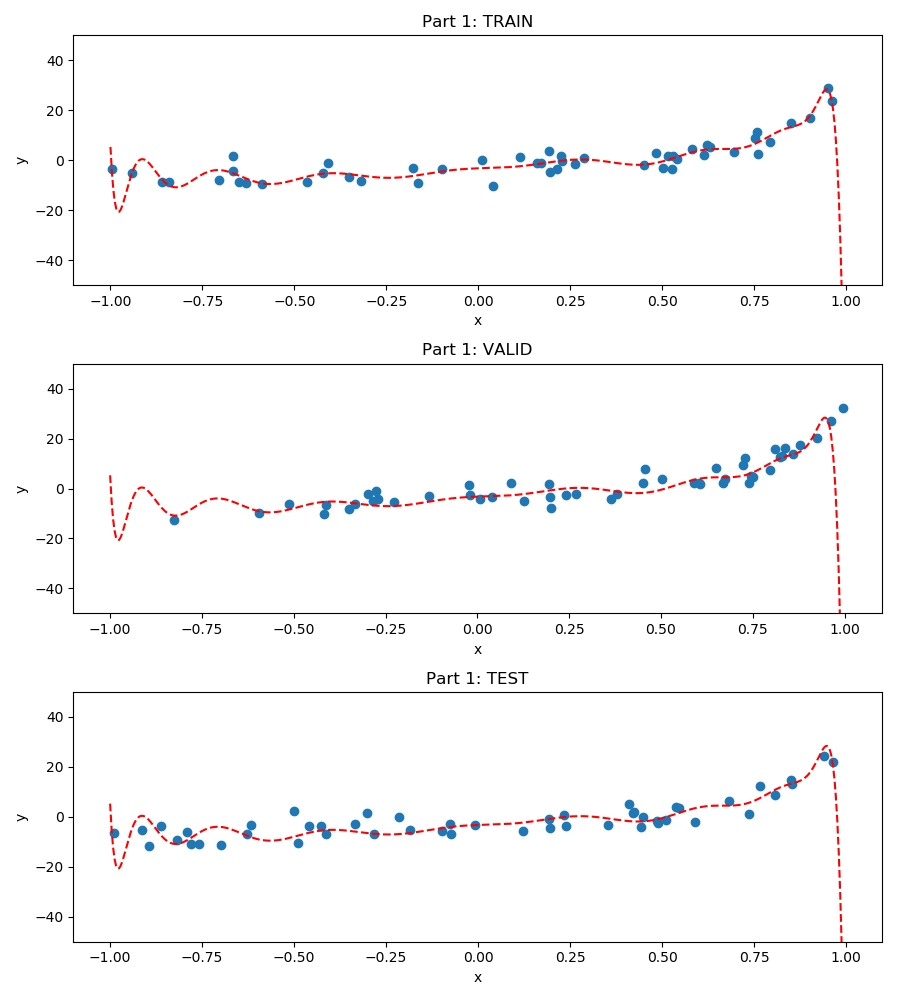
\includegraphics[width=\linewidth]{q1p1.png}
  \caption{Fit of 20-degree polynomial without regularization}
  \label{fig:q1pq}
\end{figure}


A closer look at the training plot shows oscillations of the fit (i.e. it is trying very hard to fit the training data). This observation, along with a high validation MSE of 458.64632 indicates that the 20-degree polynomial overfits the dataset. In other words, while the training MSE is low, the curve does not fit the vali 

%----------------------------------------------------------------------------------------
%	PROBLEM 2
%----------------------------------------------------------------------------------------

\section{Lists}

%------------------------------------------------

\subsection{Example of list (3*itemize)}
\begin{itemize}
	\item First item in a list 
		\begin{itemize}
		\item First item in a list 
			\begin{itemize}
			\item First item in a list 
			\item Second item in a list 
			\end{itemize}
		\item Second item in a list 
		\end{itemize}
	\item Second item in a list 
\end{itemize}

%------------------------------------------------

\subsection{Example of list (enumerate)}
\begin{enumerate}
\item First item in a list 
\item Second item in a list 
\item Third item in a list
\end{enumerate}

%----------------------------------------------------------------------------------------

\end{document}
